\chapter*{Dodatak: Prikaz aktivnosti grupe}
		\addcontentsline{toc}{chapter}{Dodatak: Prikaz aktivnosti grupe}
		
		\section*{Dnevnik sastajanja}
		
		\begin{packed_enum}
			\item  sastanak
			
			\item[] \begin{packed_item}
				\item Datum: 20. listopada 2022.
				\item Prisustvovali: svi članovi tima
				\item Teme sastanka:
				\begin{packed_item}
					\item  sastanak s asistentom i demonstratorom
					\item  raščišćavanje elemenata projektnog zadatka
					\item  predaja alternativnog "Eventko" projekta
				\end{packed_item}
			\end{packed_item}
			
			\item  sastanak
			\item[] \begin{packed_item}
				\item Datum: 24. listopada 2022.
				\item Prisustvovali: svi članovi tima
				\item Teme sastanka:
				\begin{packed_item}
					\item  razrada koncepta projekta
					\item  osmišljavanje dodatnih funkcionalnosti, aktera
					\item  prijedlog podjele uloga
				\end{packed_item}
			\end{packed_item}
		
			\item  sastanak
			\item[] \begin{packed_item}
				\item Datum: 27. listopada 2022.
				\item Prisustvovali: svi članovi tima
				\item Teme sastanka:
				\begin{packed_item}
					\item  finalna podjela uloga
					\item  odabir radnog okruženja
				\end{packed_item}
			\end{packed_item}
		
			\item  sastanak
			\item[] \begin{packed_item}
				\item Datum: 3. studenog 2022.
				\item Prisustvovali: svi članovi tima
				\item Teme sastanka:
				\begin{packed_item}
					\item  instalacija potrebne programske potpore
					\item  detaljna skica funkcionalnosti stranice
					\item  daljnja podjela rada
					\item  dizajn originalnog logotipa
				\end{packed_item}
			\end{packed_item}
		
			\item  sastanak
			\item[] \begin{packed_item}
				\item Datum: 14. studenog 2022.
				\item Prisustvovali: svi članovi tima
				\item Teme sastanka:
				\begin{packed_item}
					\item  priprema za demonstraciju osnovnih funkcionalnosti
					\item  povezivanje backenda i frontenda
					\item  usklađivanje ograničenja
				\end{packed_item}
			\end{packed_item}
		
			\item  sastanak
			\item[] \begin{packed_item}
				\item Datum: 15. studenog 2022.
				\item Prisustvovali: svi članovi tima
				\item Teme sastanka:
				\begin{packed_item}
					\item  daljnja priprema za demonstraciju osnovnih funkcionalnosti
					\item  izrada UML, sekvencijskog te dijagrama razreda
					\item  dovršeno povezivanje frontenda i backenda
					\item  lokalna pohrana prijave
				\end{packed_item}
			\end{packed_item}
		
			\item  sastanak
			\item[] \begin{packed_item}
				\item Datum: 7. prosinca 2022.
				\item Prisustvovali: svi članovi tima
				\item Teme sastanka:
				\begin{packed_item}
					\item  priprema za prvo kolokviranje
					\item  izmjene dijagrama baze podataka
				\end{packed_item}
			\end{packed_item}
			
			%
			
		\end{packed_enum}
		
		\eject
		\section*{Tablica aktivnosti}

			\begin{longtblr}[
					label=none,
				]{
					vlines,hlines,
					width = \textwidth,
					colspec={X[7, l]X[1, c]X[1, c]X[1, c]X[1, c]X[1, c]X[1, c]X[1, c]}, 
					vline{1} = {1}{text=\clap{}},
					hline{1} = {1}{text=\clap{}},
					rowhead = 1,
				} 
				\multicolumn{1}{c|}{} & \multicolumn{1}{c|}{\rotatebox{90}{\textbf{Velimir Kovačić }}} & \multicolumn{1}{c|}{\rotatebox{90}{\textbf{Jakov Krčadinac }}} &	\multicolumn{1}{c|}{\rotatebox{90}{\textbf{Ana Marić }}} & \multicolumn{1}{c|}{\rotatebox{90}{\textbf{Ema Nekić }}} &	\multicolumn{1}{c|}{\rotatebox{90}{\textbf{Filip Perković }}} & \multicolumn{1}{c|}{\rotatebox{90}{\textbf{Fran Saganić }}} &	\multicolumn{1}{c|}{\rotatebox{90}{\textbf{Luka Srića }}} \\  
				Upravljanje projektom 		& 7 & 5 &  &  &  &  & \\ 
				Opis projektnog zadatka 	& 2 & 3 &  &  & 5 & 2 & \\ 
				
				Funkcionalni zahtjevi       &  &  &  &  & 2 & 1 &  \\ 
				Opis pojedinih obrazaca 	&  & 1 &  &  & 3 &  &  \\ 
				Dijagram obrazaca 			& 2 &  &  &  & 3 & 4 &  \\ 
				Sekvencijski dijagrami 		&  &  &  &  &  & 5 &  \\ 
				Opis ostalih zahtjeva 		&  & 1 &  &  & 2 & 1 &  \\ 

				Arhitektura i dizajn sustava	 & 2 & 1 &  &  & 3 &  &  \\ 
				Baza podataka				& 3 & 2 &  &  &  & 5 &   \\ 
				Dijagram razreda 			& 3 &  &  &  & 3 & 3 &   \\ 
				Dijagram stanja				&  &  &  &  & 3 &  &  \\ 
				Dijagram aktivnosti 		&  &  &  &  & 3 &  &  \\ 
				Dijagram komponenti			&  &  &  &  &  & 1 &  \\ 
				Korištene tehnologije i alati 		&  &  &  &  & 2 &  &  \\ 
				Ispitivanje programskog rješenja 	& 2 & 1 & 5 & 5 &  & 4 & 3 \\ 
				Dijagram razmještaja			&  &  &  &  &  & 1 &  \\ 
				Upute za puštanje u pogon 		& 2 &  &  &  & 3 &  &  \\  
				Dnevnik sastajanja 			&  & 2 &  &  & 3 &  &  \\ 
				Zaključak i budući rad 		& 1 & 1 &  &  & 1 &  &  \\  
				Popis literature 			& 1 &  &  &  & 1 &  &  \\  
				Izrada početne stranice 	& 1 & 1 & 4 & 3 &  &  & 3 \\
				Spajanje s bazom podataka 	& 4 &  &  &  &  &  &  \\
				Back end 					& 25 & 2 &  &  &  &  &  \\ 
				Deployment					& 9 &  &  &  &  &  &  \\ 
				Front end					&  & 12 & 24 & 24 &  &  & 32  \\
				Izrada prezentacije			&  & 3 &  &  &  &  &  \\ 
			\end{longtblr}
					
					
		\eject
		
			\section*{Dijagrami pregleda promjena}
		
			\begin{figure}[H]
				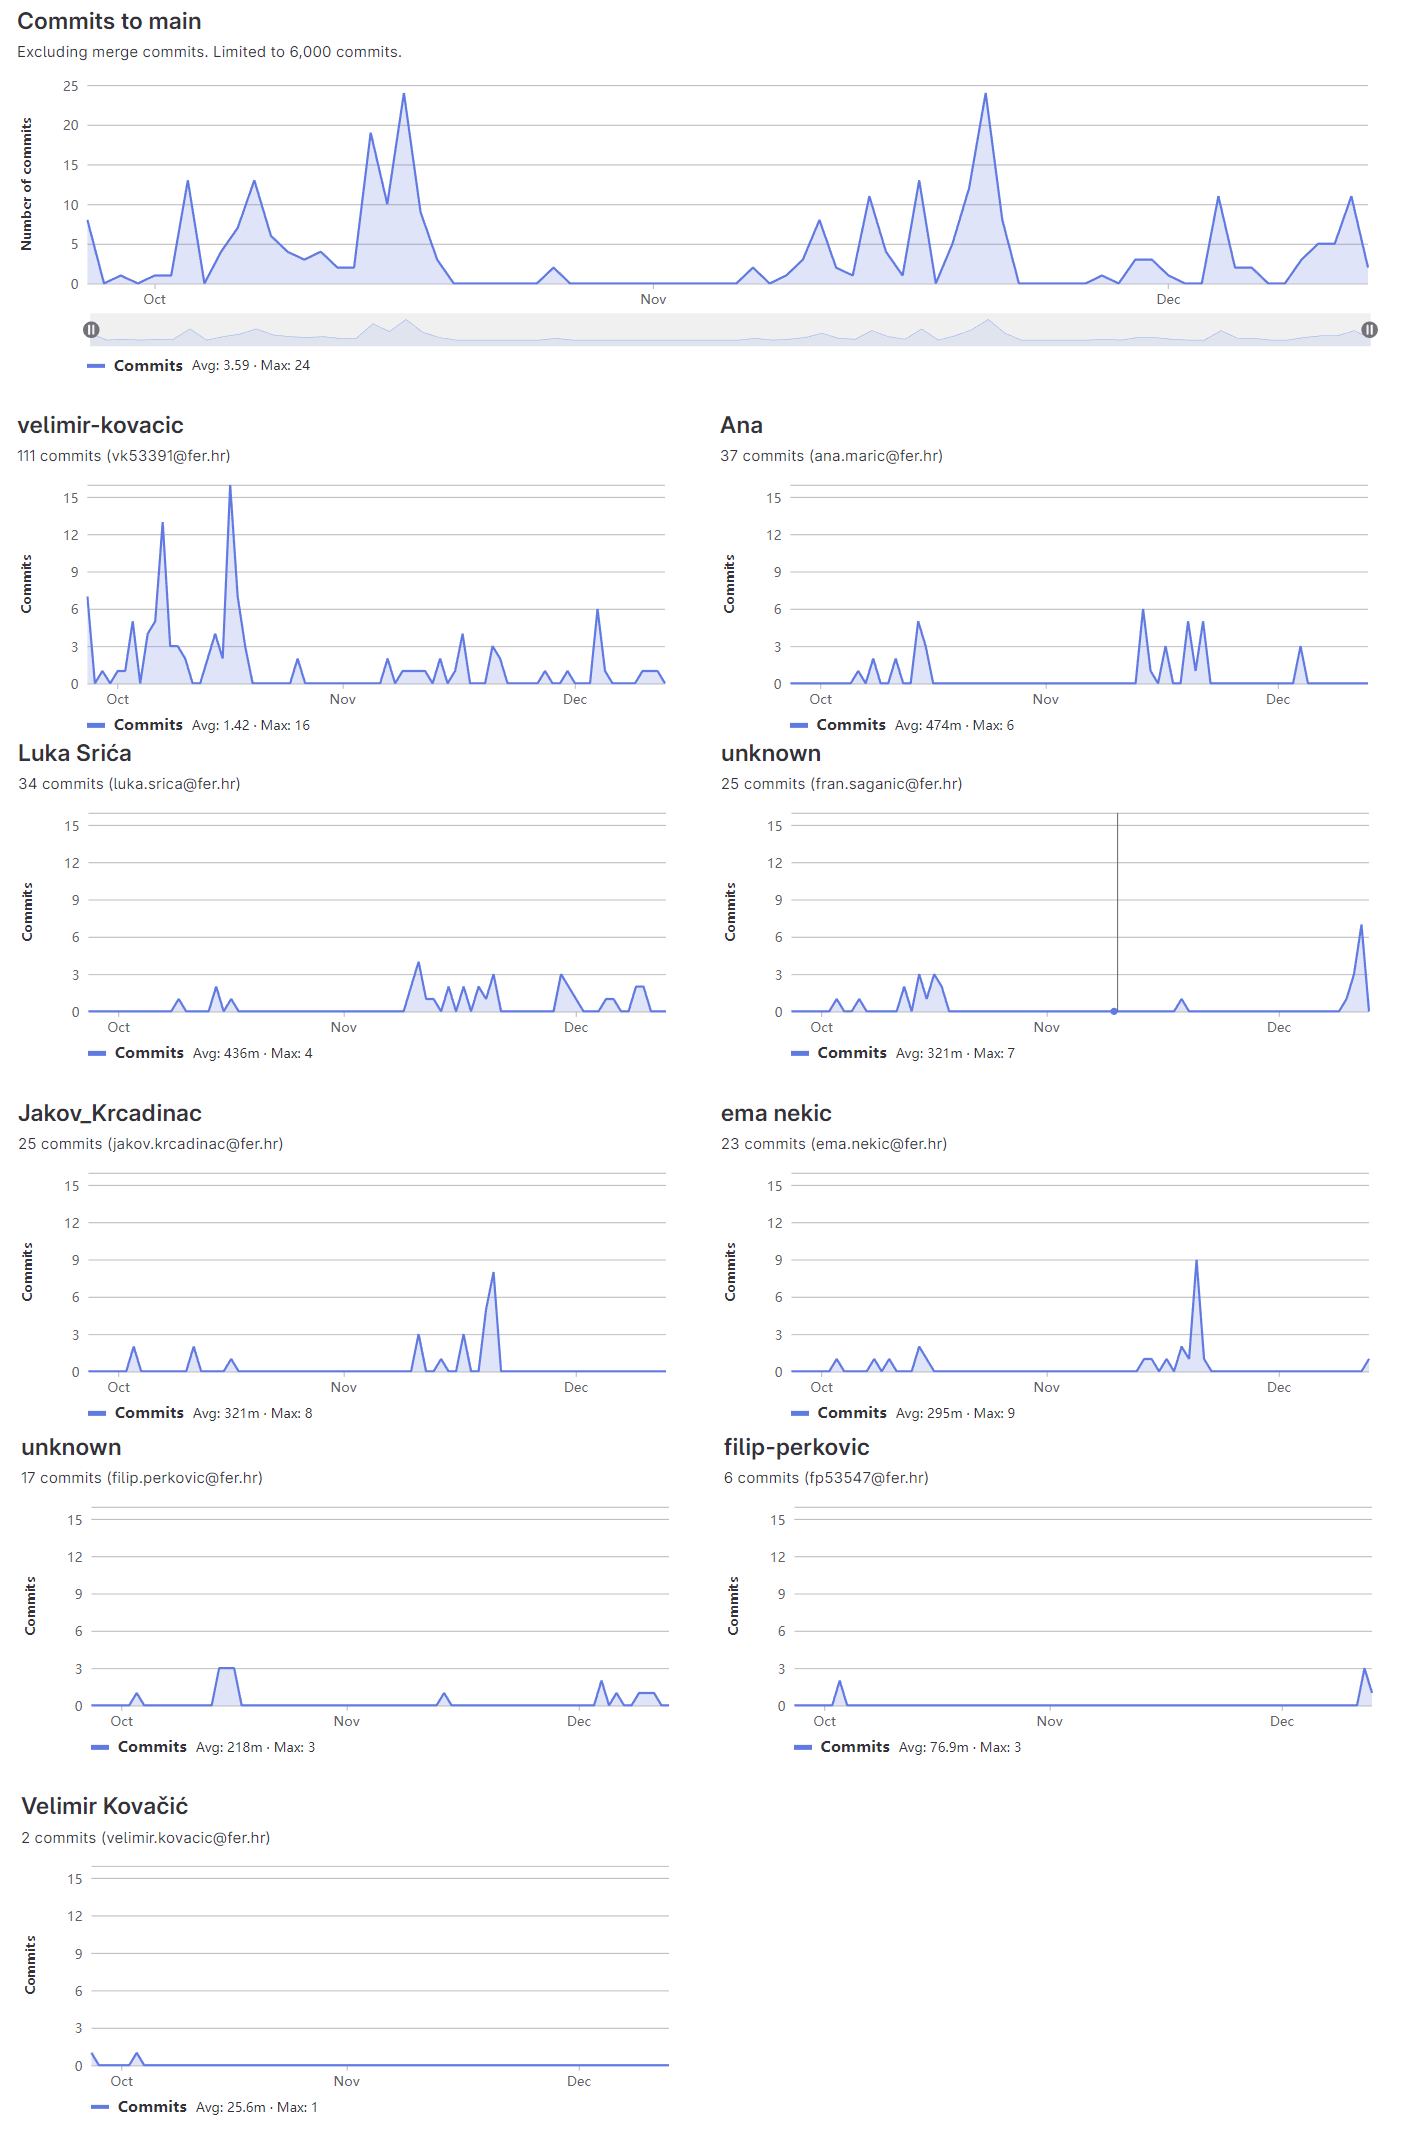
\includegraphics[height=0.85\textheight]{slike/komitovi.png}
				\caption{Grafovi aktivnosti s GitLaba}
			\end{figure}
		
	